\documentclass[acmsmall,screen,nonacm]{acmart}

\settopmatter{printacmref=false}
\setcopyright{none}
\renewcommand\footnotetextcopyrightpermission[1]{}

\usepackage{booktabs}
\usepackage{graphicx}
\usepackage{microtype}
\usepackage{tabularx}
\usepackage{tikz}
\usetikzlibrary{arrows.meta,positioning,calc}

\graphicspath{{../article_figures/}{../article_interactive/assets/}}

\title{Arithmetic Without Numbers}
\subtitle{What happens inside an LLM when it tries to calculate with nothing but matrices}

\author{Alvaro Videla}
\makeatletter
\def\@authorsaddresses{}
\makeatother

\begin{abstract}
Rune studies whether arithmetic structure inside a language model can be read
and used without parsing the prompt text. The strongest current result is an
activation-derived tool-argument route on Llama-3.1-8B: operation and operand
readouts are decoded from captured activations, then Python computes only after
the decoded tuple exists. This is not a claim of native arithmetic repair or
residual-state JIT replacement. It is a narrower result about internal
representations, provenance, and the boundary between reading a mechanism and
using it safely.
\end{abstract}

\begin{document}
\maketitle

\begin{figure}[t]
  \centering
  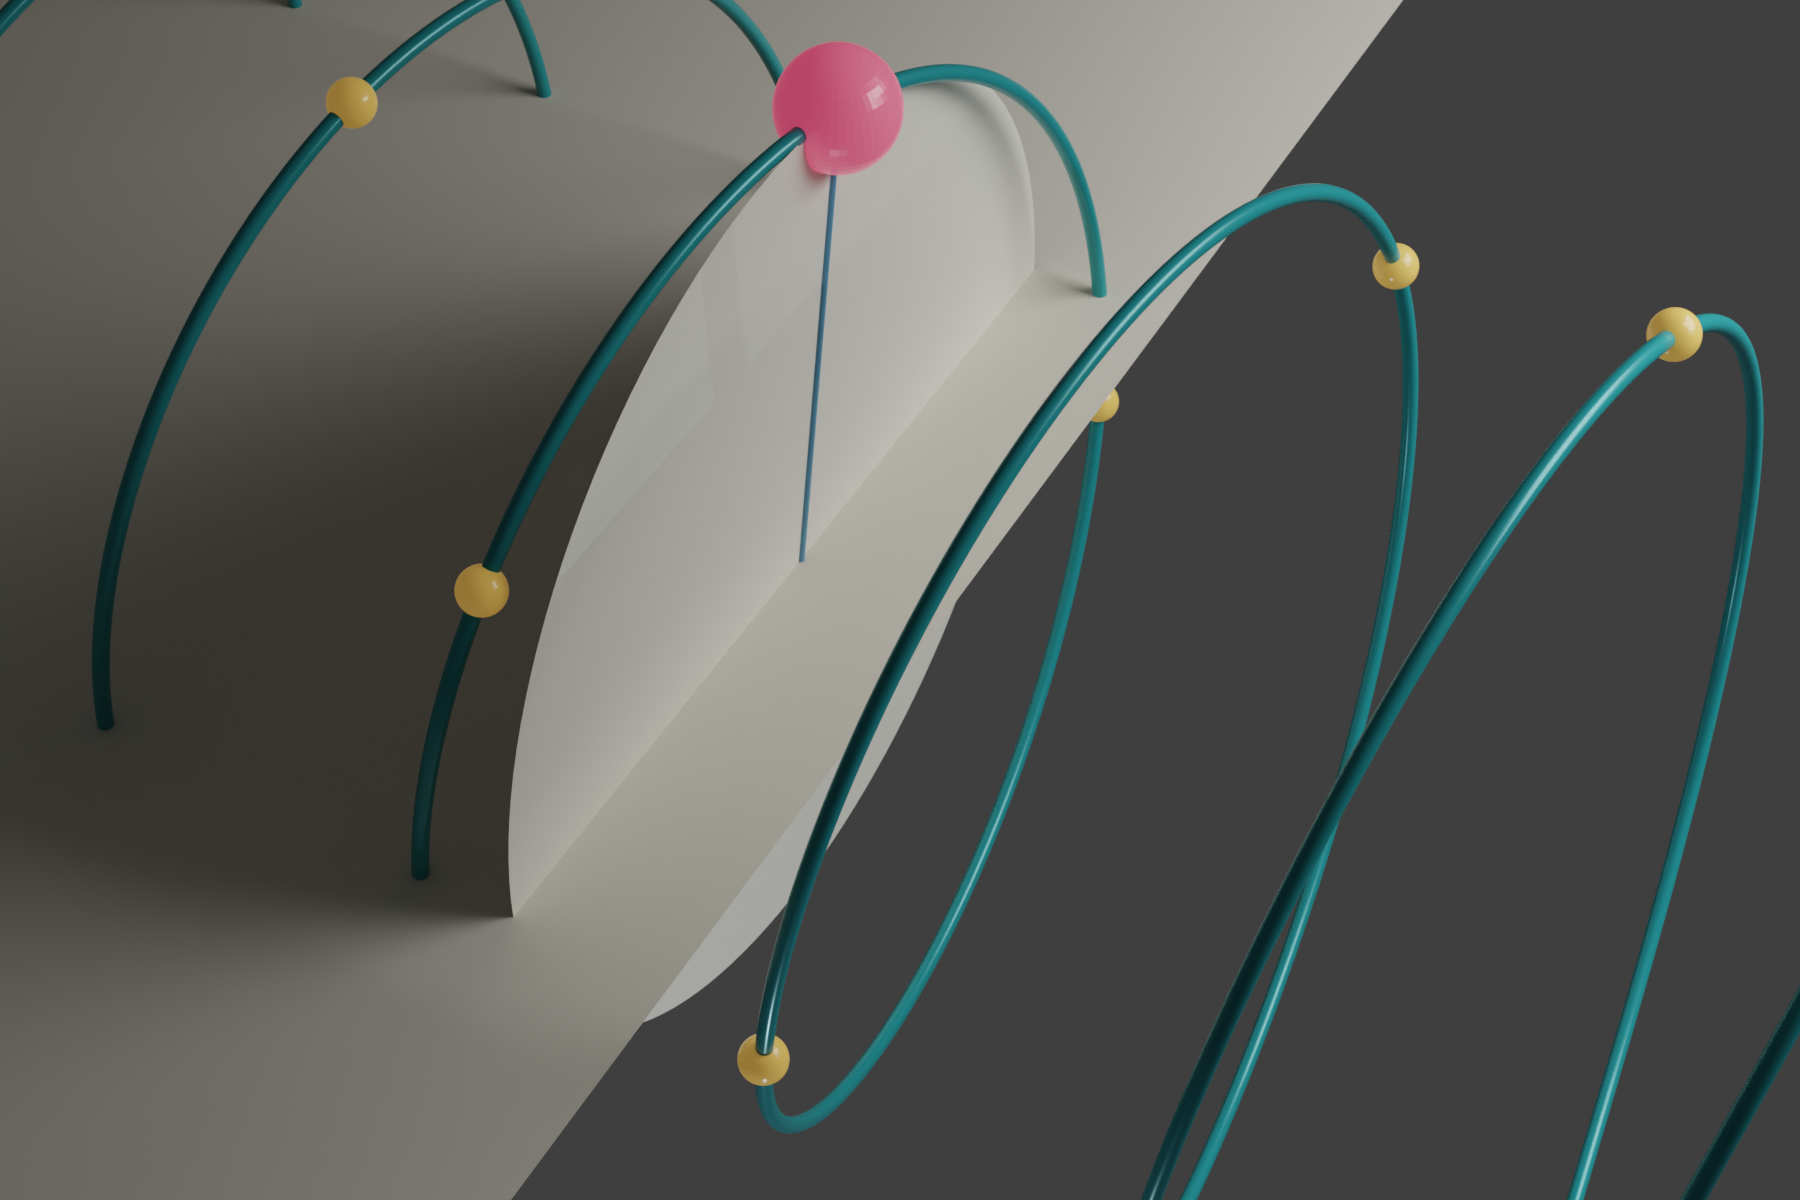
\includegraphics[width=\linewidth]{blender_integer_helix.png}
  \caption{A visual analogy for integer phase geometry in a matrix-only model:
  value can be represented by position on rotating directions rather than by
  fingers, beads, or written columns.}
  \Description{A rendered helix-like curve with glowing integer points.}
\end{figure}

\section{The Question}

If you learned arithmetic the ordinary human way, you probably learned it with
a body. You counted on fingers, grouped things into piles, lined digits into
columns, and carried a one. Human arithmetic is full of objects: fingers,
beads, marks, columns, strokes, and places.

A language model has none of that. It has matrices.

At each layer, a grid of numbers transforms another grid of numbers. Tokens
enter, activations flow, logits come out. No fingers. No abacus. No column of
digits written on a page. And yet, if you ask a modern language model for the
greatest common divisor of two numbers, or a multiplication, or a division with
remainder, something inside that matrix-only body responds.

Sometimes it answers correctly. Often it does not. The question that started
Rune was simple to ask and hard to answer: how does a language model do
arithmetic, if all it has are vectors?

The first temptation is to treat this as a product problem. If the model is bad
at arithmetic, call a calculator. That works. It is also not very mysterious. A
parser can read ``what is 84 times 37,'' translate it into \texttt{84 * 37},
send that expression to Python, and return the result. That general family of
external-computation routes is well established: PAL and Program of Thoughts
ask models to produce executable programs, ReAct interleaves reasoning with
actions, and Toolformer studies models learning when and how to call
APIs~\cite{gao2022pal,chen2022pot,yao2022react,schick2023}.

Rune was chasing a different question. Could we look inside the model and find
the calculation it was trying to perform? Could the model's own internal states
tell us the operation and operands? And, if so, could we use that information
without cheating by reading the prompt text directly?

\section{A Different Kind of Tool Use}

The original dream was more ambitious: a mechanism-aware just-in-time compiler
for model arithmetic. The ideal pipeline looked like this. The model reads an
arithmetic prompt; we identify the internal mechanism it is using; we replace
the unreliable part with exact computation; then the model continues naturally,
as if it had done the math itself.

That is a beautiful idea. It is also not what Rune proves.

What survived the experiments was narrower, but more interesting than ordinary
tool use. In a frozen Llama model, internal activations expose enough structure
to recover the arithmetic operation and operands under a strict no-parser rule.
The runtime is not allowed to use regexes, prompt text, hidden labels,
command-line operands, or gold answers. It gets token IDs and activations. From
those activations, it must infer: this is gcd, or lcm, or multiplication, or
division with remainder; these are the two numbers. Only after that decoded
tuple exists may Python compute.

The calculator is not the surprising part. The surprising part is that the
arguments to the calculator can come from inside the model.

That distinction matters because a normal tool route can solve the problem
without learning anything about model internals. Rune asks whether the model's
residual stream already carries the calculation description, even when the
model's own next-token answer would be wrong.

\begin{figure*}[t]
  \centering
  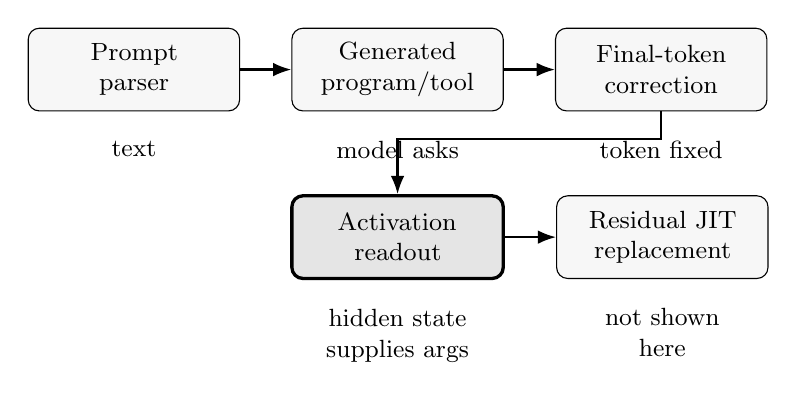
\begin{tikzpicture}[
    font=\small,
    box/.style={draw, rounded corners, align=center, minimum height=1.05cm,
      text width=2.45cm, fill=black!3},
    active/.style={draw, rounded corners, align=center, minimum height=1.05cm,
      text width=2.45cm, fill=black!10, very thick},
    arrow/.style={-Latex, thick}
  ]
    \node[box] (p) {Prompt\\parser};
    \node[box, right=0.65cm of p] (tool) {Generated\\program/tool};
    \node[box, right=0.65cm of tool] (logit) {Final-token\\correction};
    \node[active, below=1.05cm of tool] (read) {Activation\\readout};
    \node[box, right=0.65cm of read] (write) {Residual JIT\\replacement};
    \draw[arrow] (p) -- (tool);
    \draw[arrow] (tool) -- (logit);
    \draw[arrow] (logit.south) -- ++(0,-.35) -| (read.north);
    \draw[arrow] (read) -- (write);
    \node[align=center, below=0.25cm of p] {text};
    \node[align=center, below=0.25cm of tool] {model asks};
    \node[align=center, below=0.25cm of logit] {token fixed};
    \node[align=center, below=0.25cm of read] {hidden state\\supplies args};
    \node[align=center, below=0.25cm of write] {not shown\\here};
  \end{tikzpicture}
  \caption{Claim ladder for the same visible answer. Rune's supported claim is
  the highlighted activation-readout route: the calculator arguments come from
  hidden vectors, not from prompt parsing or an already-known answer.}
  \Description{A five-step left-to-right claim ladder highlighting activation
  readout.}
\end{figure*}

\section{The Matrix Body}

George Lakoff and Rafael N{\'u}{\~n}ez argued that human mathematics is built
from embodied experience: grouping, moving, measuring, collecting, and
balancing~\cite{lakoff2000}. A transformer has a different body. Its body is
matrices, residual streams, attention maps, and learned projections. If human
arithmetic can grow out of fingers and spatial metaphors, what kind of
arithmetic grows out of a matrix-only body?

Recent mechanistic work suggests a geometric answer. Kantamneni and Tegmark
argued that language models can represent integers on generalized helices and
use trigonometric structure for addition~\cite{kantamneni2025}. Stolfo,
Belinkov, and Sachan used causal mediation analysis to study arithmetic
mechanisms in transformers~\cite{stolfo2023}. Other work, including Nikankin
and colleagues' ``bag of heuristics'' account, warns that model arithmetic is
often not a clean schoolbook algorithm but a mixture of learned features and
prompt-sensitive heuristics~\cite{nikankin2024}.

Rune builds on that line rather than originating it. The contribution here is a
scoped reproduction-and-extension story around activation-derived tool
arguments, provenance controls, and resolution limits. We found Fourier-like
readouts and value-like states, but also brittleness, prompt sensitivity, and
failures that look less like a perfect algorithm than a finite-resolution
internal geometry.

\subsection{A Vector Changes as the Model Reads}

Imagine reading \texttt{What is the gcd of 84 and 36?} one token at a time. The
model does not create neat variables named \texttt{operand\_a} and
\texttt{operand\_b}. Each token position carries a long vector. As the prompt
passes through transformer layers, those vectors are updated repeatedly. Some
updates move information across positions: the token for \texttt{36} can affect
the state near the answer position. Other updates reshape the local state: a
direction in the vector may become more gcd-like, more operand-like, or more
answer-like.

The terms are less exotic in context. A token is one unit the model reads or
prints; for numbers it may be a chunk of digits rather than a full integer. The
activation is the temporary vector at a token position. The residual stream is
the running vector passed from layer to layer, a shared scratchpad without named
variables. Attention lets one position gather information from others; the MLP,
or feed-forward block, then reshapes that position's vector locally. At the end,
logits score possible next tokens.

This is why readouts and patches are possible at all. If operation and operands
leave traces in the residual stream, a small readout may recover them. If a
state really matters, a patch may change behavior. If a state is writable, an
intervention may guide the model. But those are increasingly strong claims, and
the vector itself does not label which claim is true.

\begin{figure*}[t]
  \centering
  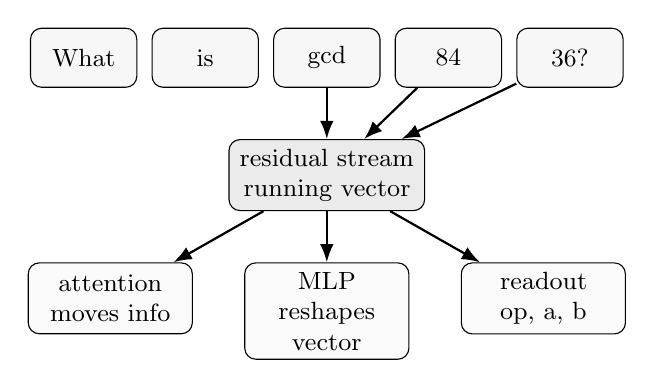
\begin{tikzpicture}[
    font=\small,
    token/.style={draw, rounded corners, align=center, minimum height=.75cm,
      minimum width=1.35cm, fill=black!3},
    state/.style={draw, rounded corners, align=center, minimum height=.9cm,
      text width=2.25cm, fill=black!8},
    op/.style={draw, rounded corners, align=center, minimum height=.9cm,
      text width=1.85cm, fill=black!2},
    arrow/.style={-Latex, thick}
  ]
    \node[token] (t1) {What};
    \node[token, right=.18cm of t1] (t2) {is};
    \node[token, right=.18cm of t2] (t3) {gcd};
    \node[token, right=.18cm of t3] (t4) {84};
    \node[token, right=.18cm of t4] (t5) {36?};

    \node[state, below=.65cm of t3] (res) {residual stream\\running vector};
    \node[op, below=.65cm of res, xshift=-2.75cm] (attn) {attention\\moves info};
    \node[op, below=.65cm of res] (mlp) {MLP\\reshapes vector};
    \node[op, below=.65cm of res, xshift=2.75cm] (readout) {readout\\op, a, b};

    \draw[arrow] (t3) -- (res);
    \draw[arrow] (t4) -- (res);
    \draw[arrow] (t5) -- (res);
    \draw[arrow] (res) -- (attn);
    \draw[arrow] (res) -- (mlp);
    \draw[arrow] (res) -- (readout);
  \end{tikzpicture}
  \caption{The residual stream is a running vector, not a named variable table.
  Attention can move operand information across positions; the MLP reshapes the
  local vector; a readout asks whether facts such as \texttt{gcd, 84, 36} are
  recoverable from that state.}
  \Description{Prompt tokens feeding a residual stream, with arrows to
  attention, MLP, and readout boxes.}
\end{figure*}

\begin{figure}[t]
  \centering
  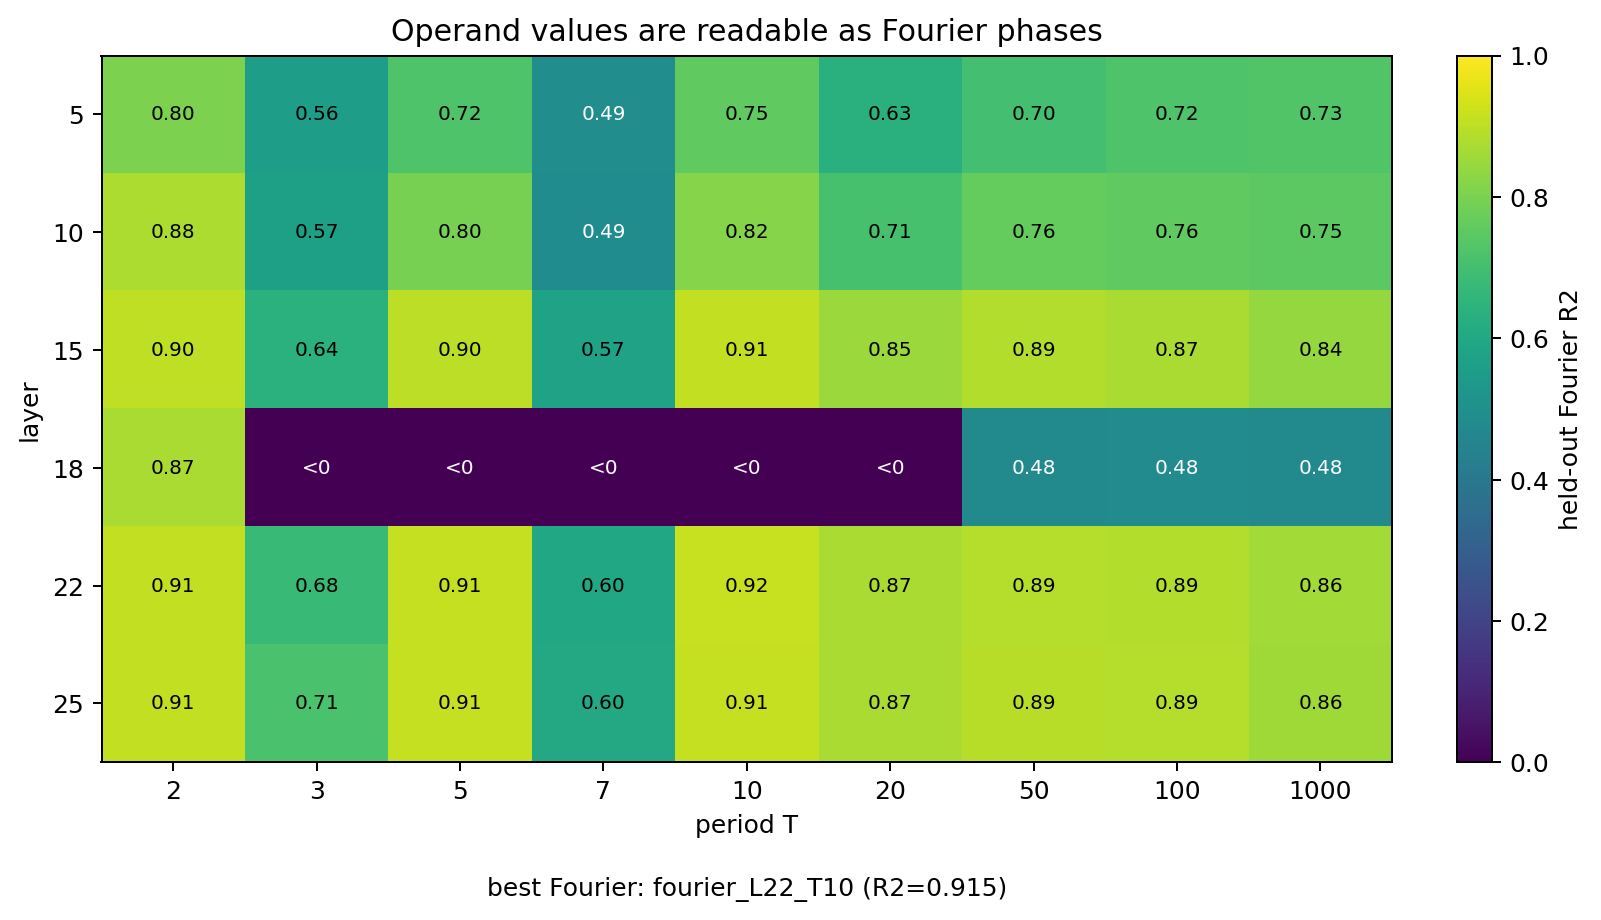
\includegraphics[width=.92\linewidth]{operand_fourier_readout_heatmap.png}
  \caption{Operand readouts are one way to ask whether number-like information
  is present in activations. A readout can show information is recoverable; it
  does not by itself prove the model used that information to compute.}
  \Description{A heatmap showing readout structure over operand Fourier
  features.}
\end{figure}

\section{Next-Token Pressure}

Next-token prediction changes the arithmetic problem. A human doing subtraction
on paper usually works from the least significant digit toward the left: units
first, then tens, then hundreds, carrying or borrowing as needed. A language
model must emit text from left to right. For the answer \texttt{15696}, it must
commit to the visible prefix before the suffix exists. In tokenized form, the
answer may come out as chunks like \texttt{15} then \texttt{696}. The model is
not filling in a scratch sheet from right to left; it is walking forward through
the string.

\begin{figure}[t]
  \centering
  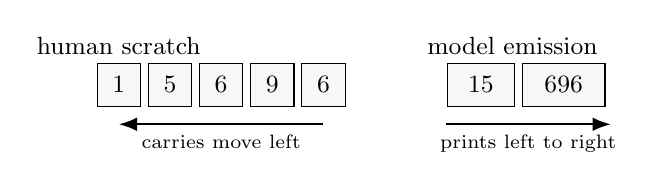
\begin{tikzpicture}[
    font=\small,
    digit/.style={draw, minimum width=.55cm, minimum height=.55cm, fill=black!3},
    arrow/.style={-Latex, thick}
  ]
    \node[align=left] at (0,1.05) {human scratch};
    \foreach \x/\d in {0/1,0.65/5,1.3/6,1.95/9,2.6/6} {
      \node[digit] at (\x,0.55) {\d};
    }
    \draw[arrow] (2.6,0.05) -- node[below] {\scriptsize carries move left} (0,0.05);

    \node[align=left] at (5.0,1.05) {model emission};
    \node[digit, minimum width=.85cm] at (4.6,0.55) {15};
    \node[digit, minimum width=1.05cm] at (5.65,0.55) {696};
    \draw[arrow] (4.15,0.05) -- node[below] {\scriptsize prints left to right} (6.25,0.05);
  \end{tikzpicture}
  \caption{Humans can compute from the rightmost digit and write the answer
  later. A next-token model must emit the visible prefix first. That makes
  numeric rendering a separate pressure from internal arithmetic.}
  \Description{A diagram contrasting human right-to-left scratch work with
  model left-to-right token emission.}
\end{figure}

That left-to-right constraint creates a rendering problem separate from the
arithmetic problem. The model may have partial information about the answer but
still lose precision as it emits longer strings. In Rune's subtraction scaling
experiment, exact greedy generation stayed at 96.7 percent for 6-digit
subtraction, fell to 63.3 percent at 10 digits, reached 53.3 percent at 13
digits, and crossed below 50 percent at 14 digits. At 24 digits it was down to
6.7 percent.

A separate counting experiment made the same pressure visible in a simpler
setting. The model saw runs of large consecutive numbers and had to print the
next one. An easy case simply advances the last chunk. A deep-carry case must
change multiple chunks at once. Cases like this collapsed; the best deep-carry
cell reached only 18.75 percent accuracy, and the dominant error was
stuck-copy.

\begin{figure}[t]
  \centering
  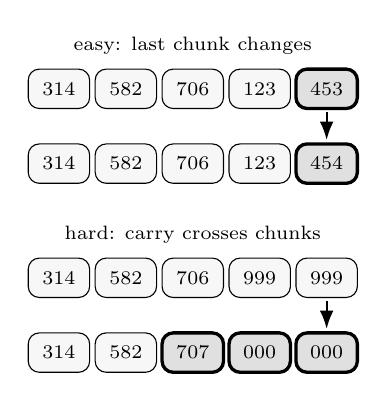
\begin{tikzpicture}[
    font=\scriptsize,
    chunk/.style={draw, rounded corners, minimum width=.78cm, minimum height=.5cm,
      align=center, fill=black!3},
    changed/.style={draw, rounded corners, minimum width=.78cm, minimum height=.5cm,
      align=center, fill=black!12, very thick},
    arrow/.style={-Latex, thick}
  ]
    \node[align=left] at (1.7,1.35) {easy: last chunk changes};
    \foreach \x/\d in {0/314,.85/582,1.7/706,2.55/123} {
      \node[chunk] at (\x,.8) {\d};
    }
    \node[changed] at (3.4,.8) {453};
    \draw[arrow] (3.4,.5) -- (3.4,.15);
    \foreach \x/\d in {0/314,.85/582,1.7/706,2.55/123} {
      \node[chunk] at (\x,-.15) {\d};
    }
    \node[changed] at (3.4,-.15) {454};

    \node[align=left] at (1.7,-1.05) {hard: carry crosses chunks};
    \foreach \x/\d in {0/314,.85/582,1.7/706,2.55/999,3.4/999} {
      \node[chunk] at (\x,-1.6) {\d};
    }
    \draw[arrow] (3.4,-1.9) -- (3.4,-2.25);
    \foreach \x/\d in {0/314,.85/582} {
      \node[chunk] at (\x,-2.55) {\d};
    }
    \foreach \x/\d in {1.7/707,2.55/000,3.4/000} {
      \node[changed] at (\x,-2.55) {\d};
    }
  \end{tikzpicture}
  \caption{The counting experiment exposed the same left-to-right pressure in
  token chunks. The easy case edits one final chunk; the hard case must update
  several chunks before the model has printed them.}
  \Description{Two chunked counting examples, one changing only the last chunk
  and one carrying across several chunks.}
\end{figure}

\begin{table}[t]
  \caption{Counting continuation example. The model tokenizer splits the
  visible number into chunks; the hard case requires a carry across two chunk
  boundaries.}
  \label{tab:counting}
  \centering
  \begin{tabularx}{\linewidth}{lX}
    \toprule
    Case & Chunks \\
    \midrule
    Easy next &
    \texttt{314 | 582 | 706 | 123 | 453 -> 314 | 582 | 706 | 123 | 454} \\
    Deep carry &
    \texttt{314 | 582 | 706 | 999 | 999 -> 314 | 582 | 707 | 000 | 000} \\
    Stuck-copy error &
    \texttt{314 | 582 | 706 | 999 | 999 -> 314 | 582 | 706 | 999 | 999} \\
    \bottomrule
  \end{tabularx}
\end{table}

\begin{figure}[t]
  \centering
  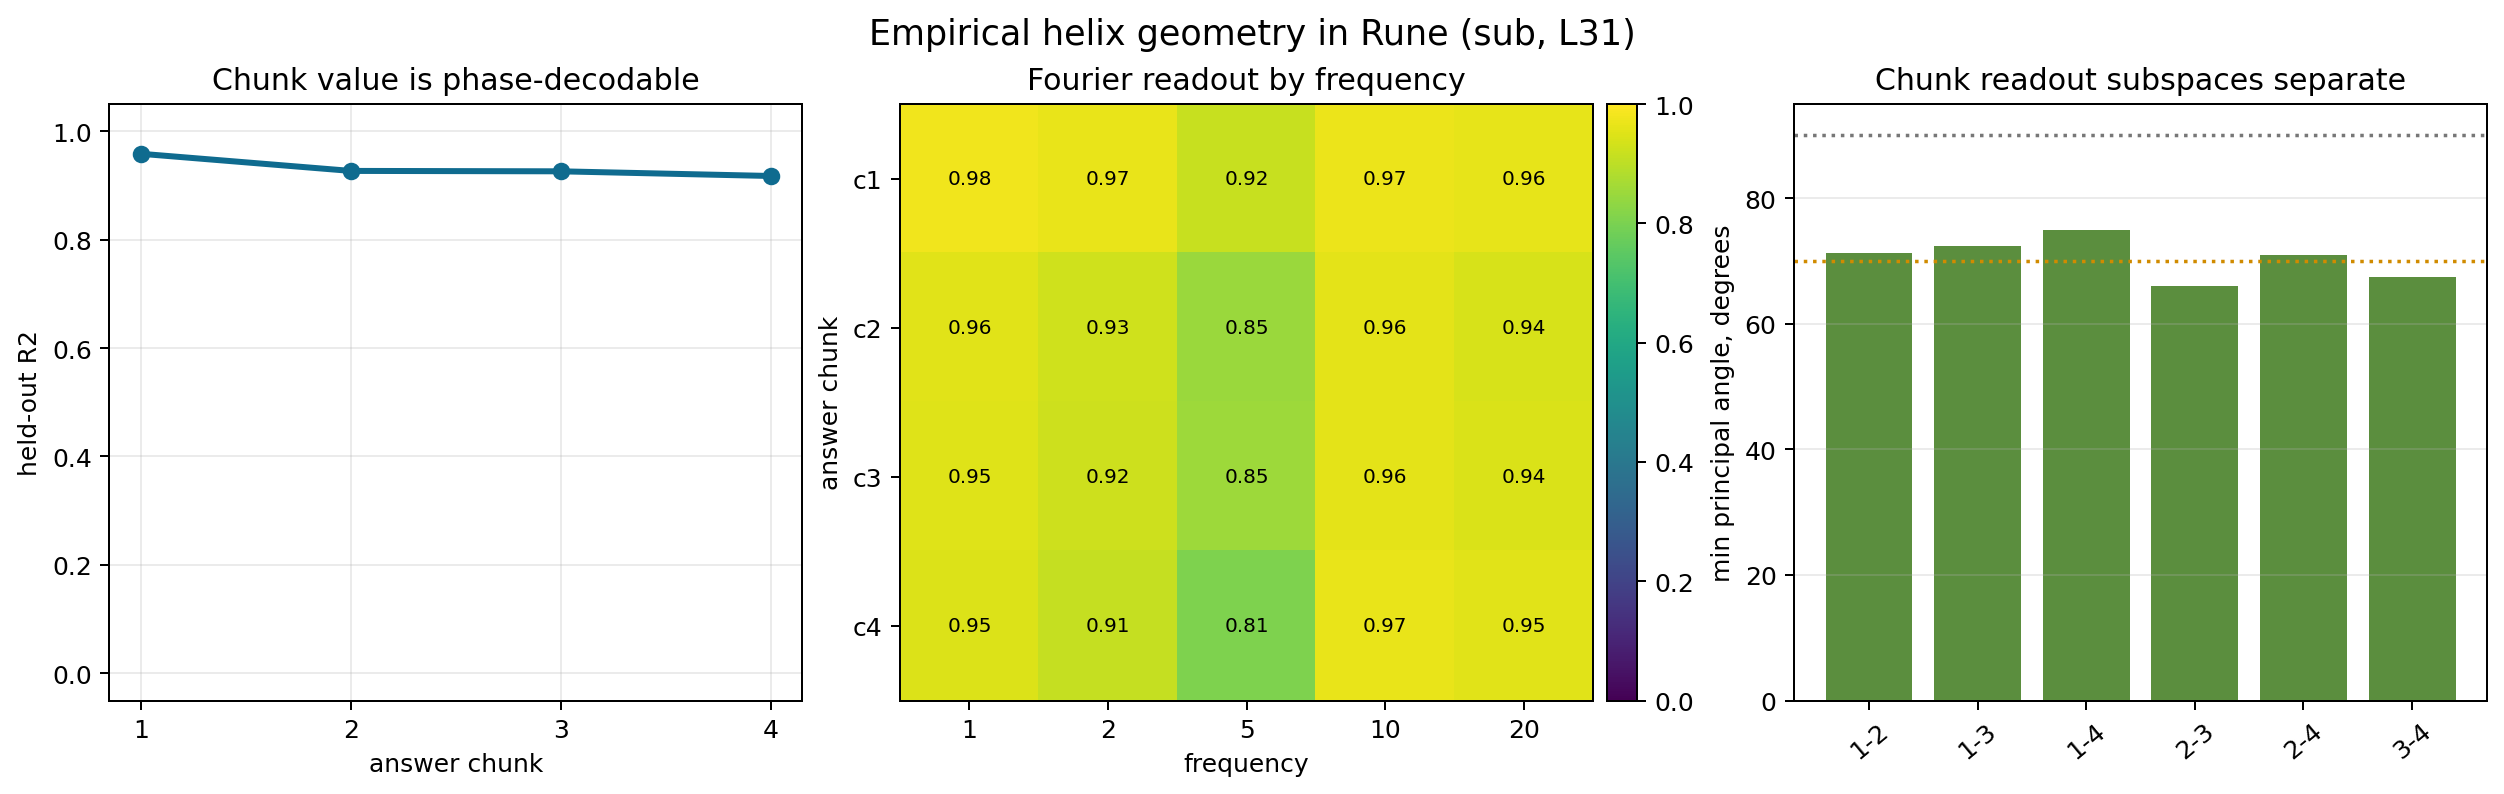
\includegraphics[width=\linewidth]{empirical_helix_resolution_sub.png}
  \caption{Empirical helix-resolution evidence for multi-chunk subtraction.
  Longer answers remain partly readable, but adjacent chunk subspaces become
  more crowded and less forgiving.}
  \Description{A plotted summary of helix resolution and chunk crowding.}
\end{figure}

The helix-resolution experiments gave a more mechanistic picture of that
boundary. For 12-digit subtraction answers split into four 3-digit chunks, each
chunk remained strongly phase-decodable at layer 31: $R^2$ was about 0.96 for
chunk 1 and about 0.92 for chunk 4. So the signal did not simply vanish. The
subtler finding was crowding. Adjacent chunk readout subspaces were not cleanly
orthogonal; the minimum principal angle dropped as low as 66 degrees. In a
14-digit, five-chunk follow-up, chunks 2--4 lost $R^2$ and adjacent angles
tightened further, for example c3--c4 went from 67.4 degrees to 58.8 degrees.
Two of three preregistered crowding predictions passed.

So ``the helix gets saturated'' is too crude, but ``there is a resolution
budget'' is fair. Longer answers still live in readable geometry, but the
geometry becomes more crowded and less forgiving.

\begin{table}[t]
  \caption{Subtraction exact-match rate by answer digit count. Source:
  \texttt{cd\_e10\_operand\_scaling}, 30 greedy generations per digit band.}
  \label{tab:digitscaling}
  \centering
  \begin{tabular}{rrrr}
    \toprule
    Digits & Exact & Prefix correct & Mean edit distance \\
    \midrule
    6 & 96.67\% & 97.2\% & 0.10 \\
    10 & 63.33\% & 80.7\% & 0.60 \\
    13 & 53.33\% & 73.8\% & 1.07 \\
    14 & 43.33\% & 67.1\% & 1.07 \\
    16 & 33.33\% & 64.6\% & 1.40 \\
    24 & 6.67\% & 17.6\% & 8.77 \\
    \bottomrule
  \end{tabular}
\end{table}

\begin{table}[t]
  \caption{Adjacent chunk subspace angles tightened in the 14-digit follow-up.
  Smaller angles mean less separation between nearby readout directions.}
  \label{tab:chunkangles}
  \centering
  \begin{tabular}{lrr}
    \toprule
    Chunk pair & 12-digit & 14-digit \\
    \midrule
    c1--c2 & 71.3$^\circ$ & 65.3$^\circ$ \\
    c2--c3 & 66.0$^\circ$ & 60.2$^\circ$ \\
    c3--c4 & 67.4$^\circ$ & 58.8$^\circ$ \\
    \bottomrule
  \end{tabular}
\end{table}

\begin{figure}[t]
  \centering
  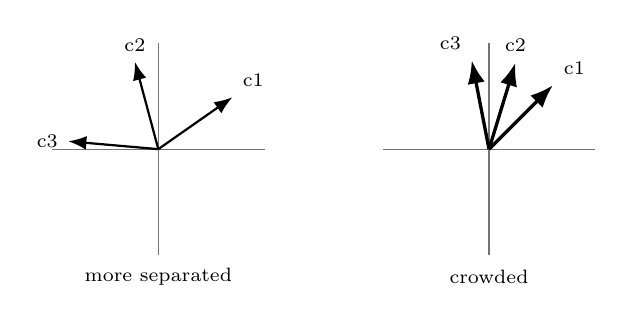
\begin{tikzpicture}[
    font=\scriptsize,
    axis/.style={draw=black!55},
    ray/.style={-Latex, thick},
    crowded/.style={-Latex, very thick}
  ]
    \draw[axis] (-1.35,0) -- (1.35,0);
    \draw[axis] (0,-1.35) -- (0,1.35);
    \draw[ray] (0,0) -- (35:1.15) node[above right] {c1};
    \draw[ray] (0,0) -- (105:1.15) node[above] {c2};
    \draw[ray] (0,0) -- (175:1.15) node[left] {c3};
    \node at (0,-1.62) {more separated};

    \begin{scope}[xshift=4.2cm]
      \draw[axis] (-1.35,0) -- (1.35,0);
      \draw[axis] (0,-1.35) -- (0,1.35);
      \draw[crowded] (0,0) -- (45:1.15) node[above right] {c1};
      \draw[crowded] (0,0) -- (73:1.15) node[above] {c2};
      \draw[crowded] (0,0) -- (101:1.15) node[above left] {c3};
      \node at (0,-1.62) {crowded};
    \end{scope}
  \end{tikzpicture}
  \caption{Crowding is a geometric resolution problem. In the experiments this
  was measured with principal angles between chunk readout subspaces; the
  drawing is only a visual guide to what smaller angles mean.}
  \Description{Two angle diagrams contrasting separated chunk directions with
  crowded chunk directions.}
\end{figure}

\section{What Failed Usefully}

At first, this looked like a path toward the compiler dream. If we could write
the right answer state into the model, perhaps the model would continue from
there.

The evidence sharpened that hope into something more modest. Making a model
emit a known answer is not the same as making the model compute. If the
experiment already knows the answer, and then uses that answer to choose a
steering vector, it has measured the model's ability to render a supplied
value. That is useful, but it is not arithmetic understanding, and it is not an
honest deployment pipeline.

This was one of the first major lessons: token rendering can masquerade as
computation.

The residual-write story also became clearer. We tried to write corrected
answer information into the model's residual stream and let it continue. For
the tested single-site writes, residual interventions had no accuracy advantage
over simpler token or logit correction. Worse, they disturbed surrounding
behavior more. That did not prove residual replacement is impossible. It proved
something more practical: a readable variable is not necessarily a writable
register.

Mechanistic interpretability often celebrates reading: decode a concept,
localize a feature, find a direction. Sparse autoencoders and dictionary
learning are one important approach to naming such features in dense activation
spaces~\cite{bricken2023,cunningham2023}. Activation patching is one common way
to move from readout toward causal evidence, but patching methodology has its
own pitfalls and metric choices~\cite{zhang2023patching}. Engineering wants an
even stronger property: change the state, preserve behavior, continue
execution. Those are different problems.

\section{The Inspection Toolbox}

Most of Rune was not one big experiment. It was a toolbox applied repeatedly,
with stricter controls each time. The tools are useful, but each answers a
different question.

This is why the article keeps distinguishing readout, causality, and writable
replacement. A probe asks, ``Can I read something?'' An SAE asks, ``Can I name
the parts?'' A patch asks, ``Does this part matter?'' Steering asks, ``What
happens if I push it?'' Confusing those questions is how interpretability
experiments accidentally overclaim.

\begin{figure*}[t]
  \centering
  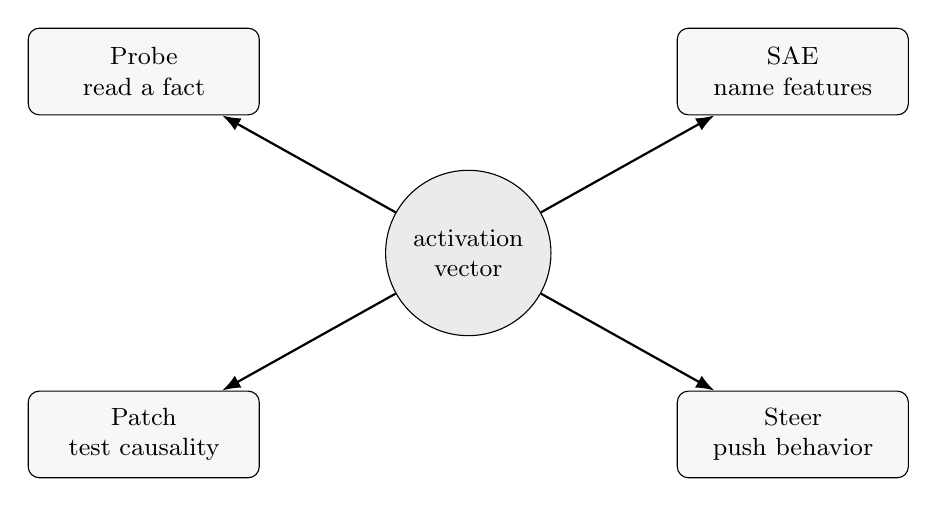
\begin{tikzpicture}[
    font=\small,
    center/.style={draw, circle, align=center, minimum width=2.1cm, fill=black!8},
    tool/.style={draw, rounded corners, align=center, text width=2.7cm,
      minimum height=1.1cm, fill=black!3},
    arrow/.style={-Latex, thick}
  ]
    \node[center] (act) {activation\\vector};
    \node[tool, above left=1.0cm and 1.9cm of act] (probe) {Probe\\read a fact};
    \node[tool, above right=1.0cm and 1.9cm of act] (sae) {SAE\\name features};
    \node[tool, below left=1.0cm and 1.9cm of act] (patch) {Patch\\test causality};
    \node[tool, below right=1.0cm and 1.9cm of act] (steer) {Steer\\push behavior};
    \draw[arrow] (act) -- (probe);
    \draw[arrow] (act) -- (sae);
    \draw[arrow] (act) -- (patch);
    \draw[arrow] (act) -- (steer);
  \end{tikzpicture}
  \caption{The same activation can be inspected in different ways. The tools do
  not make the same claim: readout, feature naming, causal testing, and steering
  are different standards of evidence.}
  \Description{A central activation vector connected to probe, SAE, patch, and
  steering boxes.}
\end{figure*}

\section{The Route That Survived}

The final system used activation-only gates and operand readouts. It had to
decide when an arithmetic route was safe to fire, identify the operation,
identify the operand pair, and then call Python only after the decoded tuple was
formed. The result was evaluated on frozen benchmark slices, with thresholds
locked and provenance tracked.

\begin{figure*}[t]
  \centering
  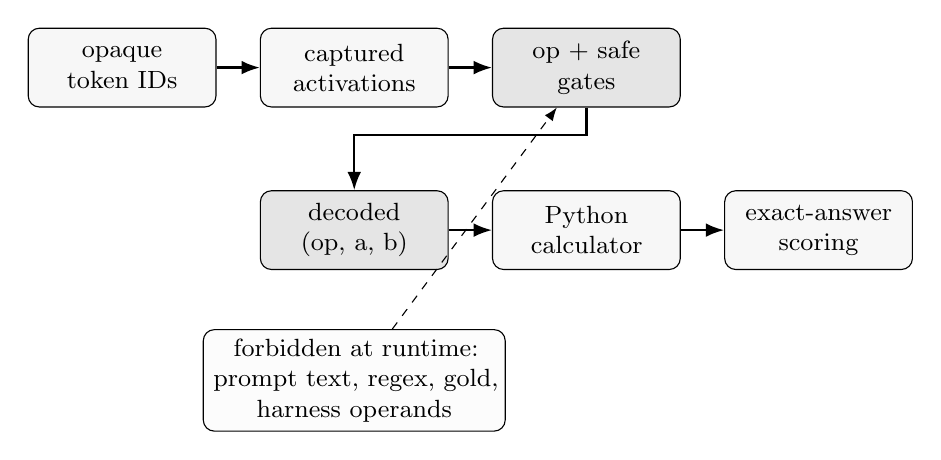
\begin{tikzpicture}[
    font=\small,
    box/.style={draw, rounded corners, align=center, text width=2.15cm,
      minimum height=1.0cm, fill=black!3},
    gate/.style={draw, rounded corners, align=center, text width=2.15cm,
      minimum height=1.0cm, fill=black!10},
    no/.style={draw, rounded corners, align=center, text width=3.6cm,
      minimum height=1.0cm, fill=black!1},
    arrow/.style={-Latex, thick}
  ]
    \node[box] (tok) {opaque\\token IDs};
    \node[box, right=.55cm of tok] (act) {captured\\activations};
    \node[gate, right=.55cm of act] (gate) {op + safe\\gates};
    \node[gate, below=1.05cm of act] (tuple) {decoded\\(op, a, b)};
    \node[box, right=.55cm of tuple] (py) {Python\\calculator};
    \node[box, right=.55cm of py] (ans) {exact-answer\\scoring};
    \draw[arrow] (tok) -- (act);
    \draw[arrow] (act) -- (gate);
    \draw[arrow] (gate.south) -- ++(0,-.35) -| (tuple.north);
    \draw[arrow] (tuple) -- (py);
    \draw[arrow] (py) -- (ans);
    \node[no, below=.75cm of tuple] (forbid) {forbidden at runtime:\\prompt text, regex, gold,\\harness operands};
    \draw[-Latex, dashed] (forbid) -- (gate);
  \end{tikzpicture}
  \caption{The surviving route is activation-derived tool use. The calculator is
  ordinary; the provenance question is whether its arguments came from hidden
  state rather than forbidden prompt-derived fields.}
  \Description{A pipeline from opaque token IDs and activations to gates, decoded
  tuple, calculator, and exact answer, with forbidden runtime fields marked.}
\end{figure*}

\begin{table}[t]
  \caption{Broad frozen arithmetic/adversarial cross-seed aggregate on
  Llama-3.1-8B. Lift is exact-answer improvement over the model's native
  answer on target prompts. False-fire is the rate of unwanted calculator calls
  on prompts where the route should stay silent.}
  \label{tab:broad}
  \centering
  \begin{tabular}{lrrr}
    \toprule
    Operation & Routed & Lift & False-fire rate \\
    \midrule
    multiplication & 0.865 & 0.852 & 0.000 \\
    division with remainder & 0.909 & 0.693 & 0.000 \\
    lcm & 0.969 & 0.966 & 0.000 \\
    gcd & 0.922 & 0.594 & 0.000 \\
    \bottomrule
  \end{tabular}
\end{table}

On a broad benchmark with the Llama weights kept frozen, the route passed across
four operations: multiplication, division with remainder, gcd, and lcm. Here
``passed'' means two things at once. On real arithmetic prompts, the route had
to fire: a gate had to decide that the calculator was allowed to run, and the
operation and operands had to come from activations. On adversarial prompts,
written to tempt the route into doing the wrong thing, it had to stay silent.
Across 11,736 locked examples---with examples, thresholds, and scoring rules
fixed before the final aggregate---and 1,536 targets, it produced large
exact-answer lifts with zero fires on the constructed hard-negative suite used
in this audit. A hard negative is a deliberately tricky no-fire prompt: it may
contain quoted arithmetic, code, a table of numbers, or an instruction saying
not to compute, but the correct behavior is no calculator call
(Table~\ref{tab:broad}).

On a recognized source slice from the DeepMind Mathematics Dataset of Saxton
and colleagues~\cite{saxton2019}, the result covered three operations: gcd,
division with remainder, and lcm. Recognized means the audit could map a dataset
prompt to one of the supported forms: two integer operands, a supported
operation, and a checkable answer. It is a coverage filter, not a claim that
every DeepMind prompt was understood or supported. Multiplication was not
claimed there because the source filtering did not produce enough accepted
two-integer multiplication examples for a powered result. Across 3,822 locked
examples and 1,233 targets, the activation-derived route again produced strong
exact-answer lifts with zero recorded false fires.

\begin{table}[t]
  \caption{Recognized DeepMind source slice. The route calculated many more
  exact answers than the frozen model produced by itself.}
  \label{tab:deepmind}
  \centering
  \begin{tabular}{lrr}
    \toprule
    Operation & Routed exact & Exact-answer lift \\
    \midrule
    division with remainder & 0.992 & +0.810 \\
    gcd & 1.000 & +0.502 \\
    lcm & 0.980 & +0.968 \\
    \bottomrule
  \end{tabular}
\end{table}

\begin{table*}[t]
  \caption{Examples of the fire/no-fire boundary. The route should fire on
  arithmetic requests, but not merely because arithmetic-looking text appears.}
  \label{tab:promptexamples}
  \centering
  \begin{tabularx}{\textwidth}{XX}
    \toprule
    Should fire & Should not fire \\
    \midrule
    \texttt{Calculate the highest common factor of 5924 and 1024.} &
    \texttt{She wrote 'gcd(48, 18) = 6' on the whiteboard and then changed the
    subject to budgets of 200 and 300.} \\
    \texttt{What is the remainder when 7696 is divided by 5130?} &
    \texttt{A reporter typed '144 / 12' into her notes but the story was about
    a basketball game.} \\
    \texttt{What is the smallest common multiple of 4740 and 1152?} &
    \texttt{The chart showed 6, 12, 18, 24 as factor labels but the article
    discussed musical notation.} \\
    \bottomrule
  \end{tabularx}
\end{table*}

The safety and provenance work mattered as much as the benchmark lifts. The
word provenance is doing real work here: it is the audit trail for where the
calculator arguments came from. We ran a full replay audit over 15,558 runtime
bundles, excluding forbidden fields such as prompt text, regex outputs, decoded
token spans, harness operands, operation labels, and gold answers. The route had
to reproduce from allowed runtime artifacts. It passed with zero replay
failures.

We also ran an independent hard-negative audit, using no-fire cases generated
separately from the positive arithmetic benchmark. The categories included
quoted arithmetic, do-not-compute prompts, wrong-operation prompts with the same
numbers, tables, logs, code, invoices, distractor-heavy number text, decimals,
signs, and out-of-domain cases. Across 10,200 non-trigger examples, the route
did not fire.

\begin{table}[t]
  \caption{Independent hard-negative audit. These are prompts where the desired
  behavior is no calculator call. Zero fires is therefore a good result inside
  this scoped audit.}
  \label{tab:hardneg}
  \centering
  \begin{tabular}{lr}
    \toprule
    Category & Fires / examples \\
    \midrule
    decimals, signs, out of domain & 0 / 1200 \\
    distractor-heavy number text & 0 / 600 \\
    do-not-compute prompts & 0 / 1200 \\
    quoted arithmetic & 0 / 1200 \\
    tables, logs, code, invoices & 0 / 2400 \\
    wrong operation, same numbers & 0 / 3600 \\
    \bottomrule
  \end{tabular}
\end{table}

\section{The Boundary}

There is causal support, but it has to be said carefully. In causal interchange
tests, selected internal operand chunks could be patched from donor examples
into recipient examples, and the decoded operands and routed calculator answers
followed the donor. This uses the same broad causal-intervention discipline as
activation patching and causal mediation work, not a new causal methodology
invented here~\cite{stolfo2023,zhang2023patching}. It supports the claim that
those internal chunks are causally involved in the decoded tuple. In the final
DeepMind causal summary, division with remainder cleared the powered pair-count
gate. Gcd and lcm had perfect rates in the available pairs, but too few pairs
to clear the frozen causal gate. So the causal evidence is supportive, not
fully powered across every final operation.

The cross-model story is also humbling. A real Qwen operand-localization sweep
failed. The current Llama route did not transfer. That is not a footnote. It is
a lesson: internal activation routes are not portable like text parsers. A
parser sees the same string. A model's internal geometry may be entirely
different.

The next steps are concrete: build model-specific operand localizers instead of
assuming transfer; complete causal interchange tests where source coverage
allows it; compare any residual-write attempt against boring logit and parser
baselines; and keep the no-parser replay boundary as a non-negotiable test.

The final claim is deliberately modest: a frozen Llama model's activations can
supply operation and operand arguments for an exact calculator under an opaque,
no-parser runtime on the current benchmark slices.

That is not native arithmetic repair. It is not a general cross-model result.
It is not behavior-preserving residual JIT compilation. But it is a useful
boundary. It shows that the model's hidden state can contain the calculation
even when its output would be wrong. It shows that mechanistic interpretability
can contribute to tool systems, if the provenance rules are strict enough. And
it shows how easy it is to overclaim unless the experiment is designed to catch
you.

\section{What To Take Away}

Models really do build arithmetic-shaped internal structure. Not arithmetic as
humans experience it, with fingers and written columns, but arithmetic as a
geometry of directions, rotations, periodic features, and value-like residual
states. A matrix-only body can invent ways to represent divisibility,
magnitude, chunks, and numeric emission.

Reading those structures is easier than turning them into a robust system. A
probe can look good for the wrong reason. A steering vector can render an
answer without proving computation. A residual write can change a token while
damaging the model's state. The interesting science is not the first positive
result; it is the sequence of controls that survives.

Tool use has layers. The easy layer is text-driven: parse the prompt, call the
tool. The harder layer is activation-derived: prove that the tool arguments
came from the model's internal state. The hardest layer is internal
replacement: write the result back into the model and preserve behavior. Rune
does not solve the hardest layer. It makes progress on the middle one.

If you want to build systems from those traces, do not trust the first
beautiful signal. Ask what else it could be measuring. Remove the prompt text.
Remove the labels. Replay without the forbidden fields. Add the annoying
negatives. Compare against the boring baseline. Separate what the model
represents from what you can safely write.

That is how the story gets smaller. It is also how it becomes true.

\bibliographystyle{ACM-Reference-Format}
\bibliography{rune_matrix_arithmetic_article}

\end{document}
